\documentclass[11pt]{article}
%Gummi|065|=)
\title{\textbf{Gravitational N-body Simulation in MATLAB}}
\author{Alexander Johansson\\
		Jarl Gullberg\\
		Karl Brorsson\\
		\\
		The Masters Programme in Spaceflight Engineering\\
		Lule\'a University of Technology\\SE-971 87 Luleå, Sweden}
\date{\today}

\usepackage{wrapfig}
\usepackage{listings}
\usepackage{mathtools}
\usepackage[utf8]{inputenc}
\usepackage{graphicx}
\usepackage{subfig}
\usepackage[export]{adjustbox}
\graphicspath{{Images/}}
\usepackage[backend=biber,style=numeric,bibencoding=utf8]{biblatex}
\addbibresource{bibliography.bib}

\begin{document}
\maketitle

\begin{abstract}
N-body simulations are a classic computational problem for physicists and programmers. The simulation of 
an arbitrary number of bodies in a gravitational system is exponentially more taxing for the computational 
hardware it runs on as the number of bodies grow, and the accuracy of the simulation suffers if the simulation
stepping is too low.

This report describes an implementation of a simple n-body simulation on a 2D plane written in MATLAB, which 
implements some common optimizations of realtime simulations. Additionally, the simulation exploits the 
object-oriented capabilites of MATLAB to improve code organization and implementation clarity.
\end{abstract}

\pagebreak
\tableofcontents

\pagebreak
%------%
\section{Preface}
This report, written in LaTeX, exists to explain the why and how this rather small program was created by us, Alexander Johansson, Jarl Gullberg and Karl Brorsson, October 2016, Luleå.

%------%
\section{Introduction}
As to why this program was created, or rather its purpose, to simulate, in a 2D plane, the effects of which gravity have on celestial bodies that do/do not have a central gravitational point, what their new point in the 2D plane is, their ne acceleration, their new direction and what happens when two, or more, bodies collides with each other.

%------%
\section{Theory}
The basic principle of a simulation is rather simple - a set of logical rules which determine how the 
simulation will progress, and a set of mathematical theories (in the form of implemented formulae) which
serve to explore the intended science of the simulation.

Each works in tandem to, over time, create a simulation of available data as reasonable close to the real 
world as possible.
\subsection{Logic Flow}
In every turing-complete programming language, there exists a set of conditional and logical constructs
which can be used to direct the path of the program through the source code (colloquially referred to as \emph{control flow statements}). 

MATLAB, which falls inside this set of languages, defines every required statement. A complete study of each is, however, beyond the scope of this report, and it is sufficient to mention their use.

For almost every simulation, the application of these statements and constructs follows a very similar structure. There is a main \emph{loop} which drives the simulation forward one batch of calculations at a time, and a set of control flow statements inside it which determine what specific calculations are made.

The shell of a simulation might look something like this:
\pagebreak
\begin{lstlisting}[language=Matlab, tabsize=4, numbers=left, frame=shadowbox]
stopCondition = false;
while(!stopCondition)
	computationFinished = doComputation();
	
	if (computationFinished)
		stopCondition = true;
	end
end
\end{lstlisting}
This simulation will run indefinitely until the computation (whatever it might be) is finished, as indicated by
the result of the \verb|doComputation| function, which in turn flips the \verb|stopCondition| and terminates the 
simulation. This is, of course, a simplifed example with exaggarated control flow for clarity.

\subsection{Gravitational Theory}
According to Newton each body is pulling on all other bodies with a force, the force is based upon the mass of the bodies and the distance between them.\\

$F = G \cdot \frac{this.m \cdot other.m}{d^{2}}$
where $G = 6.67408^{-11}$\\

Since the simulation is based on a two-dimensional plane we could use a system where each object is assigned an x and y coordinate. This allows us to use the Pythagorean theorem to calculate the distance \\

$d = \sqrt{(other.X - this.X)^{2} + (other.Y - this.Y)^{2}}$.\\

We are also required to use a mass assigned to the bodies which is the area with a density of 5.5
$m = this.Radius^{2} \cdot \pi \cdot 5.5$\\



\subsubsection{Conservation of momentum}
When two or bodies bodies collide the direction of the force and the force momentum change, the conservation of force. And since the bodies absorb one another, and it's not elastic, the conservation of momentum follows as such
$m_{1} \cdot u_{1} + m_{2} \cdot u_{2} = (m_{1} + m_{2} \cdot v$
where $m$ is the mass of the bodies, $u$ is the speed of respective body and $v$ is the speed after

%------%
\pagebreak
\section{Method}
It was clear from the beginning that, within the confines of the excercise, the bulk of the simulation would be done in a series of conditional loops wherein each object calculated the effect of each other body upon itself. Additonally, we chose to implement the simulation using MATLAB's capacity for object-oriented programming which lends itself well to a simulation with a large (and variable) number of entities (in our case, the gravitational bodies) with identical properties but variable data.

The general structure of the program follows the basic skeleton outlined in the theory, as seen in the adjacent diagram. Before the main loop, a setup phase creates an array of gravitational bodies (hereafter referred to as \emph{instances}) using constraint values collected from the user or defined by passing parameters to the simulation function.

Once past the setup stage, our main loop (in this case, a while loop) consumes the array of generated instances, which it performs simulations upon. This loop continues until only one body remains in the simulation. 

\subsection{Program Structure}
\begin{wrapfigure}{r}{0.5\textwidth}
	\vspace{-12pt}
	\begin{center}
    	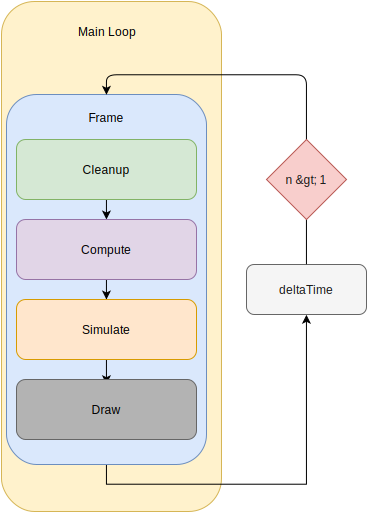
\includegraphics[scale=0.40]{MainLoopDiagram}
    \end{center}
    \caption{Program Overview}
\end{wrapfigure}

The main loop is divided into a short conditional block which governs the termination of the simulation, and a frame function.
This frame function performs four distinct phases in the simulation - cleanup, compute, simulate and draw. The cleanup phase is one of two optimizations of the simulation, which alleviates performance problems for large computations. During the cleanup phase, the program goes through the provided list of instances, checks for any instances which have merged with others (as indicated by the \verb|IsAlive| property being set to false), and removes these from processing.

After this phase, the simulation enters the compute phase where the acceleration vector of each body is determined. These values are then passed on to the simulate phase. The mathematical operations of these phases are  explained in more detail in \ref{gravityComputeInfo}. 

The simulate phase takes the previous values and applies them over a small amount of time. The smaller this step is, the more accurate the simulation is. However, it takes a longer time and requires more processing power. In its most basic form, this simulation step is subject to changes in the hardware it runs on. If left unchecked, the simulation will finish sooner and with more steps on faster processors, effectively altering the end result. Any collisions between bodies during the simulation phase cause them to merge into one, and adopt a new common position weighted by the mass of the larger body.

In order to combat this (and maintain a consistent result across different types of hardware), the time taken to complete each frame is recorded and used to modify the simulation length of the following one. This is a simple yet effective implementation of $\delta t$ frame-time, a technique most often seen in games and realtime rendering.


\subsection{Gravitational Bodies as Objects}
In order to better represent a number of logically similar (identical properties, same functionality, etc) but computationally divergent (different positions, different sizes, dissimilar states, etc), MATLAB and object-oriented languages allows you to define \emph{classes}. In essence, these act as blueprints from which you can create instances of the described object.

We created a class describing a gravitational body by its most primitive data. Excluding more complex shapes, a spherical body or particle can be reduced to just two values - a radius $r$ and a position $p(x, y)$. From these values, all geometrically relevant data can be computed, and the body can be represented visually in a plane.

Of course, adding a number of other properties will simplify the process. Therefore, we decided to include two logical values which would impact the simulation and be used in optimizations, two additional positionally relevant properties, and two graphical properties which aid the drawing of the object onto the final figure.

\begin{figure}[h]
	\centering
	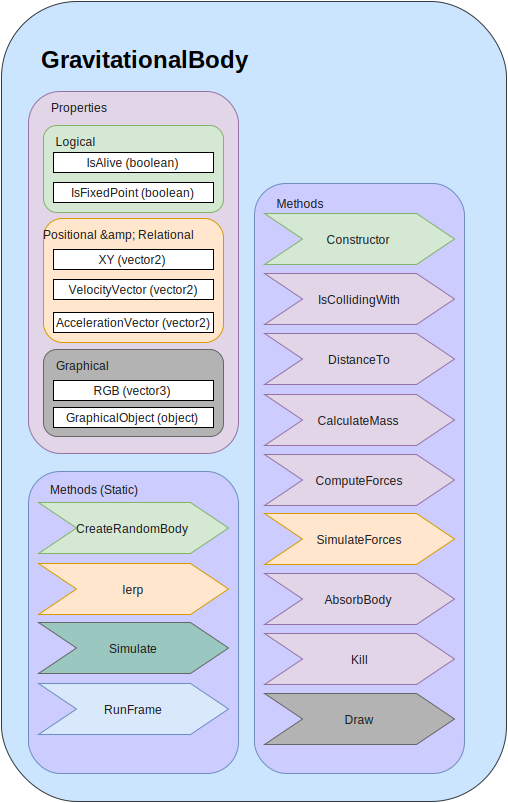
\includegraphics[scale=0.4]{GravitationalBody}
	\caption{Diagram of the GravitationalBody class}
\end{figure}

\pagebreak
\subsubsection{IsAlive}
IsAlive is a simple boolean property which is used during the cleanup phase of the simulation to determine which bodies are to be removed from the simulation and excluded from further computation. When one body collides with another, it absorbs the other and calls the \verb|Kill| function (seen above) on that body. This removes the visible shape from the simulation figure and sets this value to false.

\subsubsection{IsFixedPoint}
IsFixedPoint is an addition which, while not strictly neccesary, makes for an interesting variation on the simulation. If this value is set to true at the beginning of the simulation, all movement for this body is ignored while maintaining its effects on other bodies. In essence, this turns the simulation from a fixed viewpoint on a field of bodies into a moving viewpoint focused on this larger body and its orbiting entities. If left for enough time, all other bodies will either adopt an elliptical orbit around this fixed point or merge with it.

\subsubsection{XY}
XY is a simple positional vector storing the position of the object on the plane. The coordinates are not limited, and may take on values outside of the visible bounds of the simulation.

\subsubsection{AccelerationVector}
AccelerationVector is a 2-element vector of accelerations in the X and Y directions, and is one of the core properties of the body - here and in VelocityVector, the momentum gained in the previous frame is maintained between iterations in the simulation. This allows for cumulative simulation of forces on the bodies, replicating desired the real-world conditions. 

\subsubsection{VelocityVector}
Like AccelerationVector, this property is a 2-element vector of velocities in the X and Y directions. Velocity, like acceleration, is preserved between frames. Velocity, however, is not recalculated during each compute step like Acceleration, and is instead more strictly cumulative.
'
\subsubsection{RGB}
RGB is a 3-element vector of floating-point values which defines an RGB triplet, used in the drawing of the body on the simulation figure. This is simply the colour the object will take on when drawn. The value is randomized upon object creation.

\subsubsection{GraphicalObject}
GraphicalObject is a property born out of neccesity, and was added at a later stage in the design. This property stores an instance of MATLAB's \verb|rectangle| object, which is the visible representation of the body in the simulation. These are, due to a quirk in the way MATLAB handles figures, not affected by the typical \verb|hold on / hold off| combination and must instead be explicitly added or removed.

Beyond the properties, each body has a set of functions which are directly tied to the class (hereafter referred to as \emph{methods}). These are divided into two distinct types - static and instance methods. The static methods can be called without having an instance of the class available. An apt metaphor would be knowning the dimensions of a house - there is no need to build the house in order to find out how tall it is. All that is required is looking at the blueprint. If you, on the other hand, would like to know how old the house it, it must first have been built.

In much the same way, static methods are called without having an instance of the object, and instance methods require an instance of the object. We'll briefly look at the most important functions in the class.

\subsubsection{CreateRandomBody (Static)}
CreateRandomBody is a simple but useful function. When called with the proper limiting arguments, it creates a new instances of a gravitational body within the specified constraints. This is used in the simulation to create the initial set of bodies in a reasonably similar fashion.
\subsubsection{Simulate (Static)}
Simulate contains the actual main loop of the simulation. Due to constraints from the excercise description which neccesitated that all code be within the same file, the main loop (which would normally have been in a separate, appropriately named file) was placed in a static function on the object instead.
\subsubsection{IsCollidingWith}
IsCollidingWith takes another body as input, and determines whether or not the two bodies are colliding with each other. A simple \emph{true} or \emph{false} value is returned.
\subsubsection{CalculateMass}
CalculateMass (like the name suggests) calculates the mass of the object. This function is worth mentioning, as it is integral in the simulations and only uses the radius of the object as its dependent variable. Additionally, it takes into account the average density of a rocky body (taken as $5.5$, the avg. density of the Earth).
\subsubsection{ComputeForces}
ComputeForces takes another body as an input argument, and computes the force between the two bodies. This is done to each other body by way of the main loop, and the resulting values are then used in \verb|SimulateForces| to actually move the body.
\subsubsection{AbsorbBody}
AbsorbBody is called when two bodies collide. One body (selected by order of simulation) takes the other's mass into itself, calculates a new radius, and averages the velocity vectors to simulate a nonelastic collision where momentum is preserved.
\subsubsection{Draw}
Draw is the final step in the simulation chain. It takes the information available about the object (radius, colour and position), and uses it to draw a shape onto the visible figure. In our case, this is facilitated through the \verb|rectangle| function, which can be used to draw circles (which, in all honesty, are just rectangles with very, very round corners). The old shape is deleted, and a new one is created, drawn and stored in the instance.

\subsection{Gravitational Computation}\label{gravityComputeInfo}
The way we apply the forces is through the use vectors and objects. It first checks the position of another body (GravitationalBody) and computes a force with the help of our formula $F = G \cdot \frac{this.m \cdot other.m}{d^{2}}$ followed by the same calculation of another body not calculated before. then after the force is calculated it moves them according to the chosen timestep. this is repeated for a body until it register a collision.
\subsubsection{Computing a collision}
Through the use of a non elastic collision Matlab computes the force of the acceleration and velocity when the two bodies collides resulting with the same, increased or reduced velocity depending on the angle at the moment they collide where the force and velocity are assigned an x,y vector.

%------%
\section{Results}
What we have is what looks like a functioning gravitational simulation where we can expect where the bodies go and see that they go there. A fault in the code seems to be that the bodies flies of the screen when they shouldn't and sometimes look like they are avoiding the gravitational pull of other bodies. We assume this might be because the gravitational force is so small once the bodies are more than 10 length units away.

\begin{figure}[h]
	\centering
	\subfloat[Frame 1]{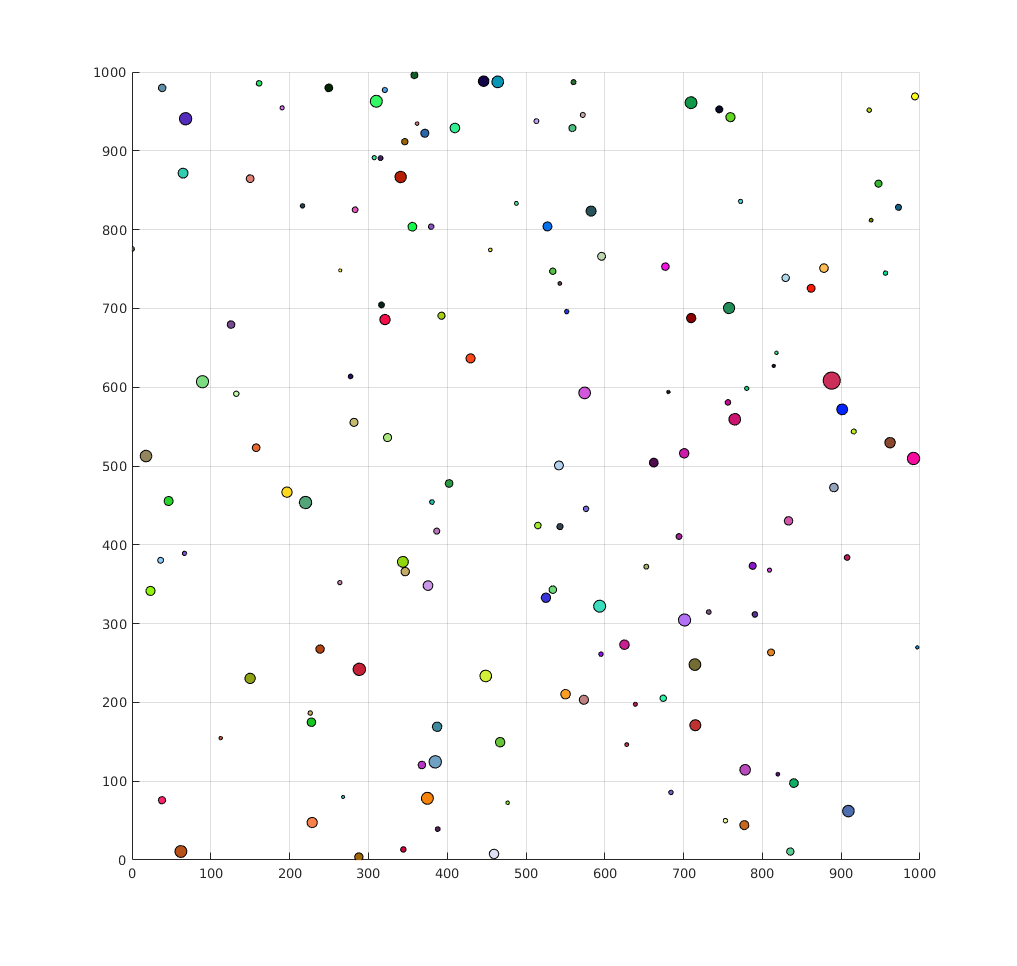
\includegraphics[scale=0.25]{frame1.png}}
	\subfloat[Frame 10]{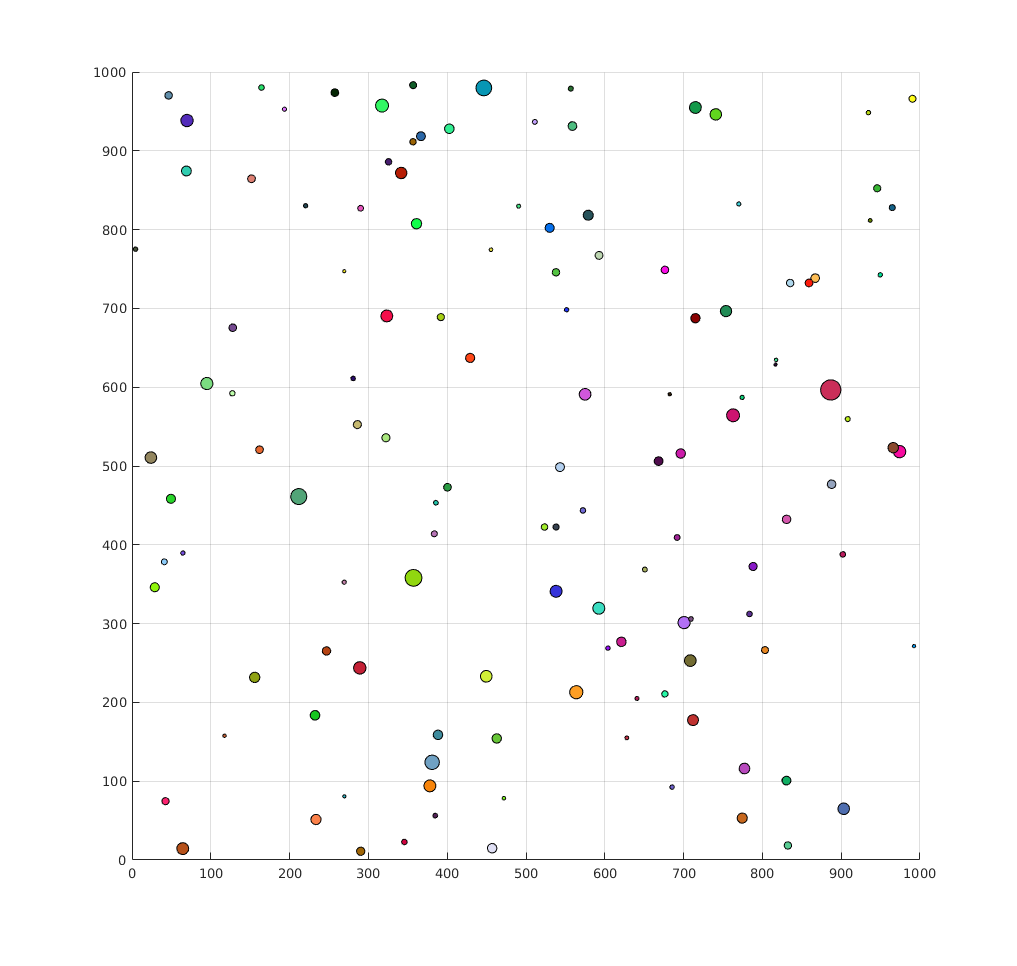
\includegraphics[scale=0.25]{frame10.png}}
	\newline
	\subfloat[Frame 20]{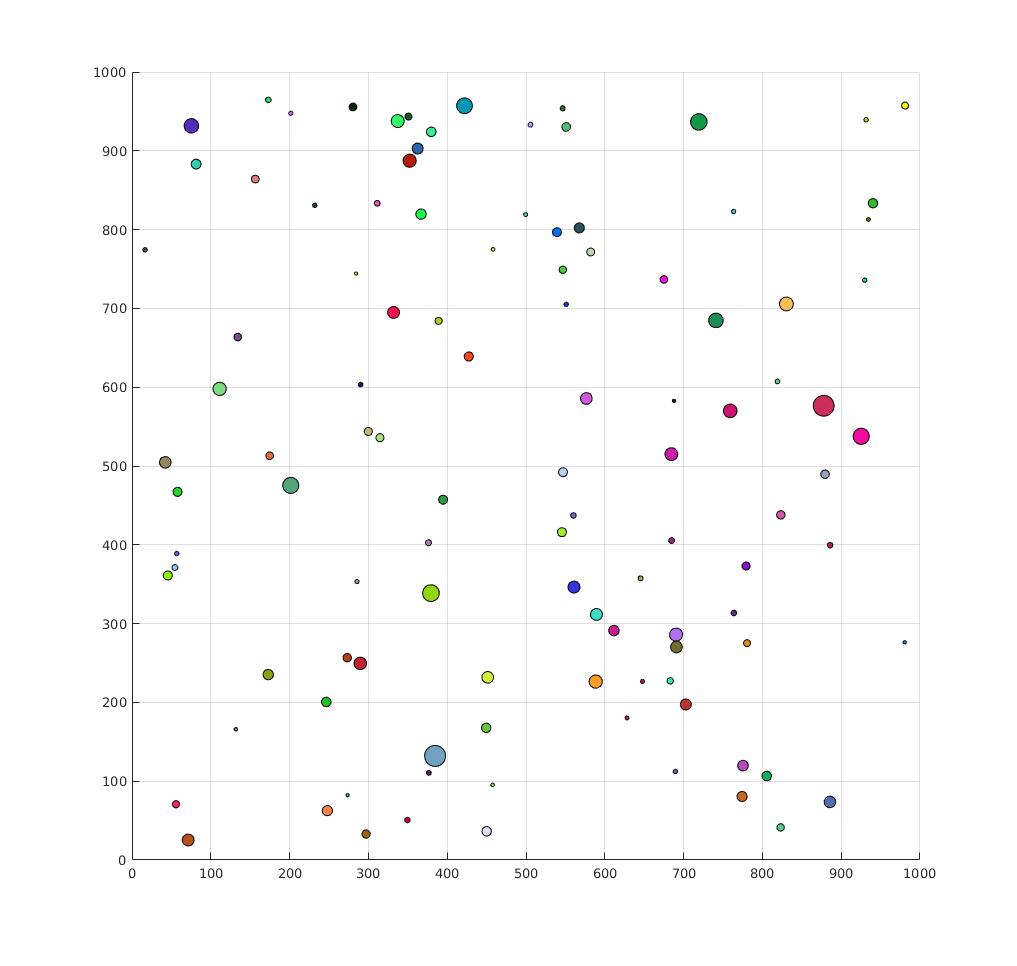
\includegraphics[scale=0.25]{frame20.png}}
	\subfloat[Frame 30]{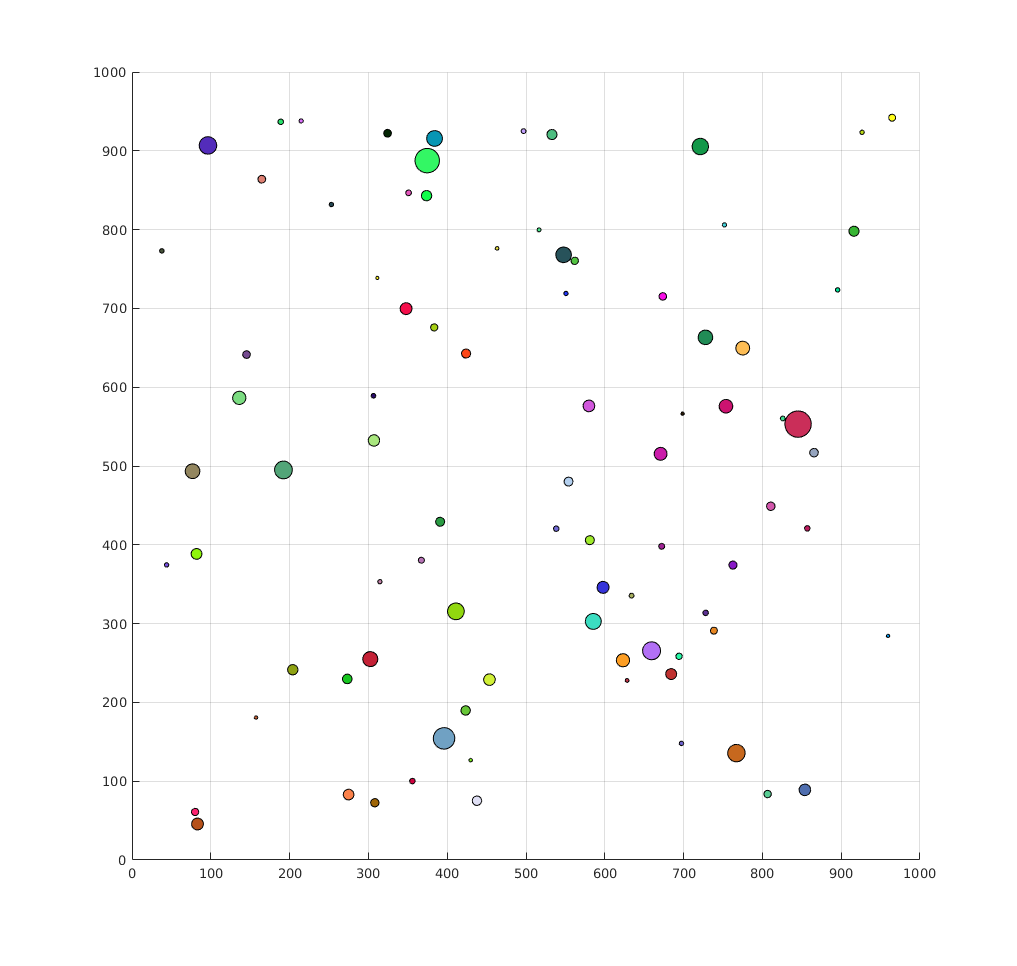
\includegraphics[scale=0.25]{frame30.png}}
	\newline
	\subfloat[Frame 100 (showing coalescing bodies)]{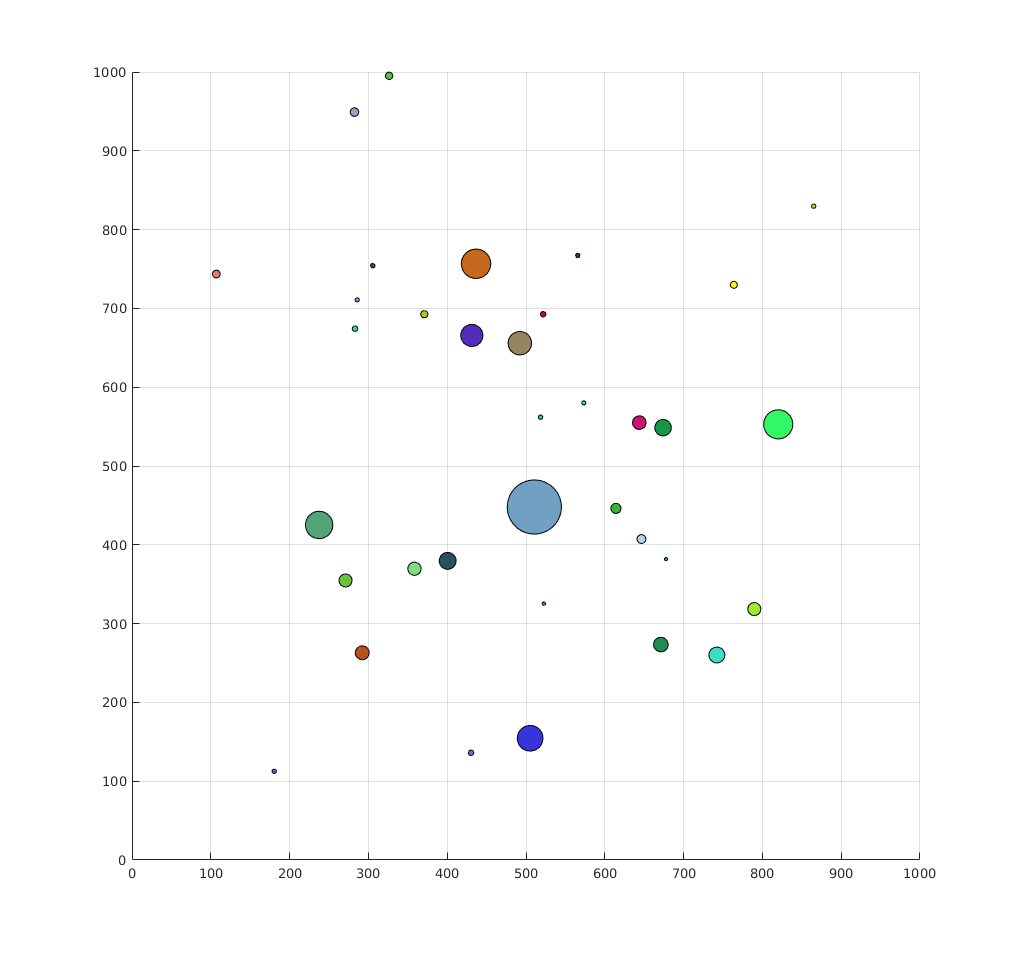
\includegraphics[scale=0.25]{frame100.png}}
	\caption{Six captures at points in the simulation}
\end{figure}

\section{Discussion}
\subsection{Goal}
The end goal with this project was to simulate the gravitational forces between celestial bodies, their new positions because of said gravitational forces, calculating their new mass from colliding with each other and their acceleration, velocity and direction after said collision, which has been reached.
\subsection{Better?}
One way to improve the simulation is to make sure that the bodies are cept inside the boundaries of the 2D plane so that the bodies will not slingshot away. Put in a counter to keep track of how many bodies are still "alive". 
\subsection{Uses}
What can this kind of program be used for? Other than smashing planets, asteroids, meteors and other celestial bodies into each other. 
It could be used for calculating a path for a satellite or a bigger spacecraft, eventually, through an asteroid field, or avoiding entire planets, maybe. 

\printbibliography

\end{document}